%----------------------------------------------------------------------------
\chapter{C-RAN koncepció}\label{sect:CranConcept}
%----------------------------------------------------------------------------
\section{Mi is az a C-RAN?}

\hspace{2mm}\cite{RecentCRANProg} \cite{Architecture} \cite{ImplementationIssues} \cite{BenefitsFujitsu} \cite{BenefitsEricsson} \cite{WirelessFull}  \cite{FutureCarrier} \cite{ImplementingGPP} \cite{NokiaSingle} \cite{TechOverview}   Az amerikai származású gépész mérnök Henry Gantt-tól származik a nevét is örző Gannt diagramm forma. Ma már a projektmenedzsment mindennapjait kiséri végig ez a feladatok ütemezését vizuálisan megragadó eszköz. Maga a diagram egy elfektetett oszlopdiagramhoz hasonlít, amelyen követhetjük a projekthez tartozó egyes feladatok elvégzésének egy ütemezését. \cite{GanttChart} Két nagyobb megjelenítendő részből áll, egy a feladatokat listázza, egy pedig a naptárszerű rész mely az elvégzési ütemtervet mutatja. 

\begin{figure}[!ht]
\centering
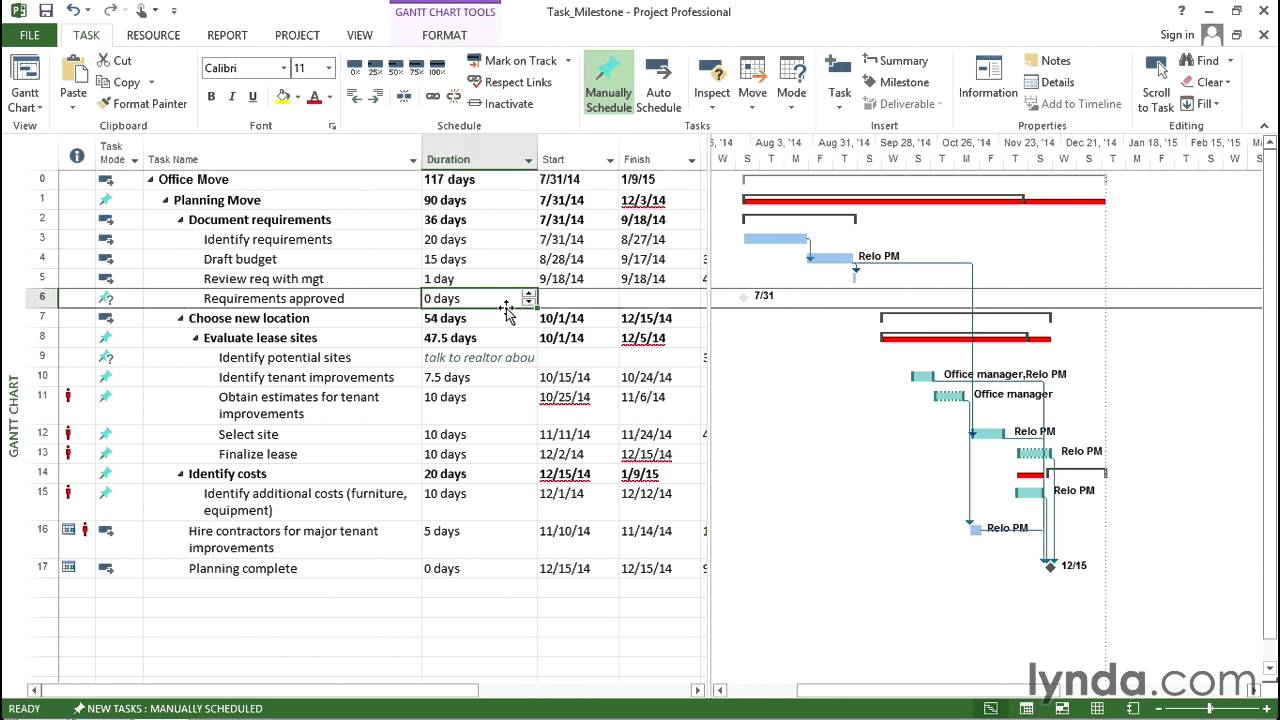
\includegraphics[width=\textwidth, keepaspectratio]{figures/msproject.jpg}
\caption{Microsoft Project 2016 Gantt program kinézete} 
\label{fig:MSProject}
\end{figure} 

A Microsoft Project által megvalósított Gantt vastag kliens alkalmazásra mutat példát a \figref{MSProject}-es ábra. Az ábrán megfigyelhetők a taskok legfontosabb tulajdonságai. Minden tasknál beállíthatjuk, hogy mennyi ideig fog tartani és, hogy milyen függöségei vannak, ezután a task kezdési és végzési idejét az alkalmazás az ütemezés függvényében állítja majd be. Láthatjuk, hogy nem csak feladatok vannak, hanem azoknak egy öszefoglalója, summaryje is melyek alá több feladat tartozhat. Fontos, hogy ez a summary nem egy külön task, hanem azoknak egy gyűjtője, az elvégzési időtartama is az alatta lévő taskok összege. Még érdemes azt is megemlíteni, hogy a program a taskok egymásutániságát nyílakkal is szemlélteti a jobb érthetőség és vizualizáció érdekében. \cite{RecentCRANProg}

A Microsoft Project ellenpontjaként több projekt próbálta vékonykliensen is megvalósítani az alkalmazást egy webes applikáció keretében, ilyen például a GanttPro, melyben a Microsoft Project legtöbb funkciója implementálásra került. A programba a \figref{GanttPro} ábra nyújt betekintést, feladatom a félév során egy ehhez hasonló alkalmazás alapjainak lefektetése volt.\cite{GanttPro}

\begin{figure}[!ht]
\centering
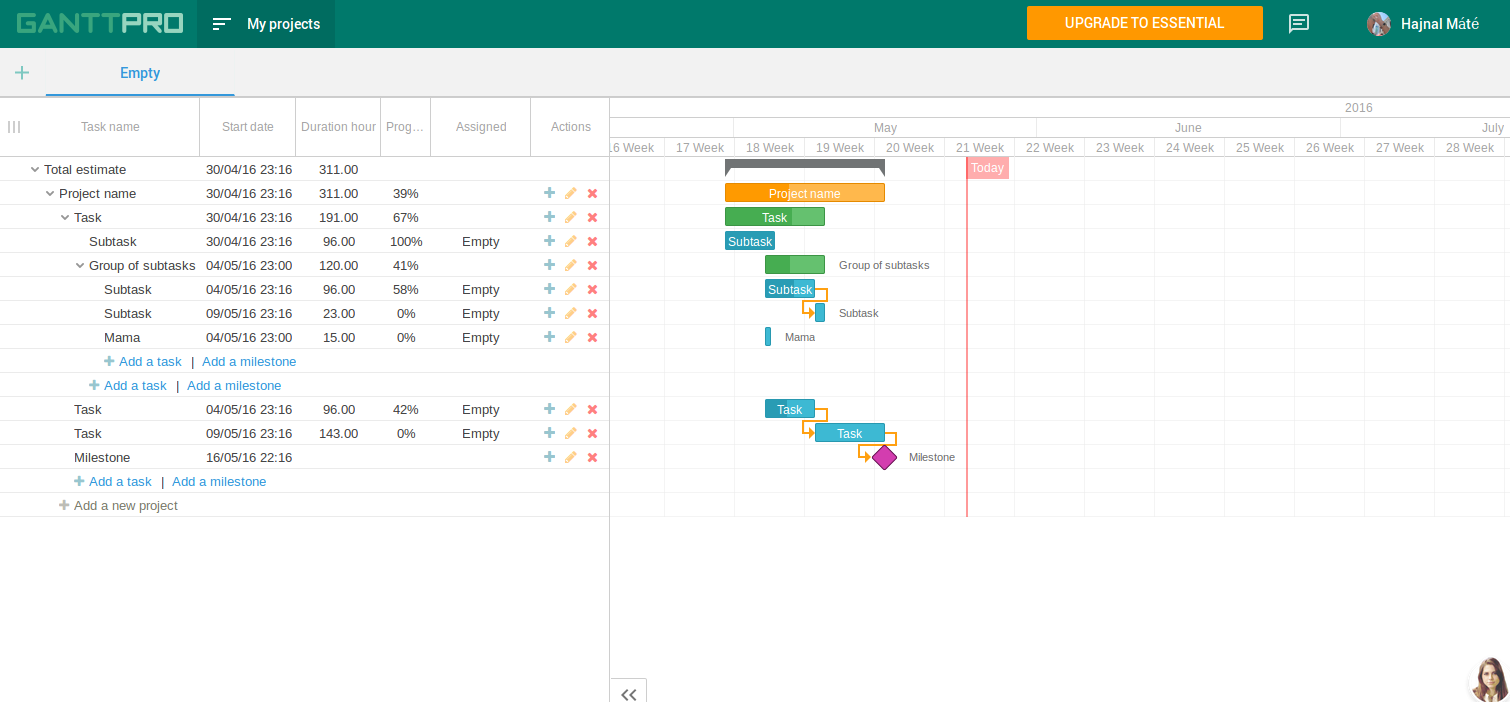
\includegraphics[width=\textwidth, keepaspectratio]{figures/ganntpro.png}
\caption{A GanttPro webes alkalmazás} 
\label{fig:GanttPro}
\end{figure} 

%----------------------------------------------------------------------------
\section{C-RAN Tulajdonságai}
\hspace{2mm} \indent Az irodalomkutatás során az első algoritmus amibe belebotlottam a Kritikus út módszer (Critical Path Method CPM). Maga a Gantt diagram inkább a megjelenítésre fókuszál, a benne lefutó algoritmusokról semmit nem mond, így ezek után az algoritmusok után kellett keresnem a félévben.  Fontos leszögeznem, hogy nincs jelenleg nem NP-nehéz tökéletes megoldása a feladatnak, így a jelenleg legelterjedtebb megoldások közül választottam. A CPM egy ilyen megoldás, mely ha előre ismerjük a feladatok végrehajtási idejét, azok erődorrásait és függőségeit, akkor segít kiszámolni a lehetséges kezdési és befejezési időpontokat. \cite{CPM}

\begin{figure}[!ht]
\centering
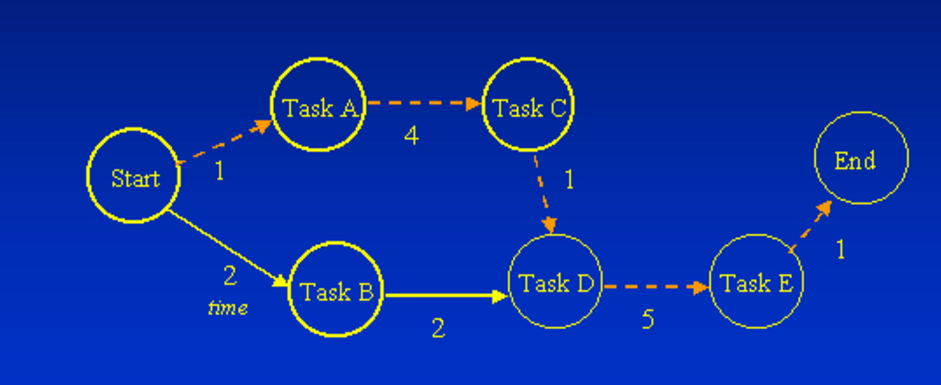
\includegraphics[width=\textwidth, keepaspectratio]{figures/cpm.png}
\caption{A Kritikus út módszerre példa} 
\label{fig:CPM}
\end{figure} 

A \figref{CPM}-es ábrán szemlélhetjük az algoritmus futását. A Start pontból indulunk és a Finish pontba szeretnénk eljutni. Az algoritmus először kiszámítja minden lehetséges útvonalra az úthosszt (ez 11 és 10), ami egy egszerű gráf algoritmust jelent, majd végül a leghosszabb útat választja, ez lesz a kritikus útvonal. Könnyen végig gondolható, hogy azért van ez így, mert a feladatok szempontjából ez az útvonal jelöli a legszűkebb keresztmetszetet, hiszen ennél hamarabb nem tudunk végezni a projekttel.

%----------------------------------------------------------------------------
\section{C-RAN Kihívásai}
\hspace{2mm}  \indent CPM-mel megtaláltuk a projektünk szempontjából legkritikusabb utat, így a végrehajtást ennek az útvonalnak a végigjárásával kell kezdenünk. Viszont a CPM  a projektben lévő többi feladat elvégzéséről nem mond semmit. Ehhez egy másik algoritmust találtam a Least Slack Time scheduling algoritmusát, azonbelül is a First verziót, mely magyarul úgy hangozhat, hogy "Legkisebb tartalékú először" algoritmus.\cite{LST} Az algoritmus lényege, hogy minden feladatnak ad egy prioritást az alapján, hogy mennyire "halogatható" (slack time) az adott feladat. A halogatási időhöz ki kell számolni minden feladatra a legkorábbi kezdési időpontot és a legkésőbbi végzési időpontot, a kettő különbsége a slack time. Ebből az előbbi a CPM algoritmusából már adódik, az utóbbit pedig úgy definiálhatjuk, mint az az időpont, amikor a feladatot legkésőbb végre kell hajtani, hogy ne legyen még csúszás a projektben. Ennek megkapásához egy újabb CPM algoritmust kell futtani úgy, hogy megfordítjuk a futás irányát, azaz a függőségeket és a kezdési időpontnak beállítjuk az utolsó feladat legkorábbi befejezési időpontját. 